
\section{Divergence and Integration by Parts}

The divergence (operator) of a differentiable vector field $v:\R^{n}\rightarrow\R^{n}$
is given by
\[
\nabla\cdot v=\sum_{i=1}^{n}\frac{\partial v_{i}}{\partial x_{i}}.
\]

\begin{example}
Consider $v(x)=(2x_{1}+x_{3}^{3},3x_{1}\sin(x_{2}),4x_{3}x_{1}^{2})$.
Then $\nabla\cdot v=2+3x_{1}\cos(x_{2})+4x_{1}^{2}$. 
\end{example}

As a special case, for twice differentiable $f:\R^{n}\rightarrow\R$,
we have the Laplacian $\Delta f\defeq\tr(\nabla^{2}f)=\nabla\cdot\nabla f$.
For a vector field $v:\R^{n}\rightarrow\R^{n}$, we have 
\[
\nabla\cdot(fv)=\nabla f\cdot v+f(\nabla\cdot v).
\]
From this, over a domain $\Omega$, we have

\[
\int_{\Omega}\nabla f\cdot v=\int_{\Omega}\nabla\cdot(fv)-\int_{\Omega}(\nabla\cdot v)f.
\]
And using the divergence theorem, namely, $\int_{\Omega}\nabla\cdot f=\int_{\partial\Omega}f\overrightarrow{n}$,
where $\overrightarrow{n}$is the normal vector at a point in $\partial\Omega$,
we have:
\[
\int_{\Omega}\nabla f\cdot v=\int_{\partial\Omega}fv\cdot\overrightarrow{n}-\int_{\Omega}f(\nabla\cdot v).
\]
The first term on the RHS become zero if the vector field $v$ goes
to $0$ at the boundary of the domain (e.g., if the domain is $\R^{n}$,
then if it decays at infinity). 

\section{Tips for Computing Gradients}

In this section, we give some tips on how to do calculus.

\subsection{Computing gradients via directional derivatives}

Usually, computing gradients coordinate-by-coordinate is not the best
way and we should avoid using summation notation as much as possible
as it creates too many subscripts and is prone to mistakes. Instead,
it is usually better to compute the gradient via directional derivatives.
Here, we give a few examples for this. We define $Df(x)[h]$ be the
directional derivative of $f$ at $x$ along the direction $h$. Namely,
\[
Df(x)[h]\defeq\left.\frac{d}{dt}\right|_{t=0}f(x+th).
\]
Similarly, we use $D^{k}f(x)[h_{1},h_{2},\cdots,h_{k}]$ to denote
the directional $k$-th derivative of $f$ at $x$ along directions
$h_{1},\cdots,h_{k}$.
\begin{lem}
Given $A\in\R^{n\times d}$. Let $\Phi(x)=\sum_{i=1}^{n}f(a_{i}^{\top}x)$
where $a_{i}$ is the $i$-th row of $A$. Then, we have $\nabla\Phi(x)=A^{\top}f'(Ax)$
and $\nabla^{2}\Phi(x)=A^{\top}\diag(f''(Ax))A$ where $f'(Ax)$ is
the vector defined by $(f'(Ax))_{i}=f'(a_{i}^{\top}x)$.
\end{lem}

\begin{proof}
Note that
\begin{align*}
D\Phi(x)[h] & =\sum_{i=1}^{n}f'(a_{i}^{\top}x)a_{i}^{\top}h,\\
D^{2}\Phi(x)[h,h] & =\sum_{i=1}^{n}f''(a_{i}^{\top}x)(a_{i}^{\top}h)^{2}.
\end{align*}
To write it in the traditional form, we note that
\begin{align*}
\nabla\Phi(x)^{\top}h & =D\Phi(x)[h]=f'(Ax)^{\top}Ah=(A^{\top}f'(Ax))^{\top}h.
\end{align*}
Since both side are the same for all $h$, we have $\nabla\Phi(x)=A^{\top}f'(Ax)$.

Similarly, we have
\begin{align*}
h^{\top}\nabla^{2}\Phi(x)h & =D^{2}\Phi(x)[h,h]\\
 & =\sum_{i=1}^{n}(f''(Ax))_{i}(Ah)_{i}^{2}\\
 & =h^{\top}A^{\top}\diag(f''(Ax))Ah.
\end{align*}
Since $\nabla^{2}\Phi(x)-A^{\top}\diag(f''(Ax))A$ is symmetric and
both side are the same for all $h$, we have $\nabla^{2}\Phi(x)=A^{\top}\diag(f''(Ax))A$.
\end{proof}
\begin{xca}
Use the above method to compute the gradient and Hessian of $f(X)=\log\det A^{T}XA$.
\end{xca}

Here is a more complicated example.
\begin{lem}[Brachistochrone Problem]
Let $(x,u(x))$ be the curve from $(0,0)$ to $(1,-1)$ where the
first coordinate is the $x$ axis and the second coordinate is the
$y$ axis. Suppose that this is the curve that takes the shortest
time for a bead to slide along the curve frictionlessly from $(0,0)$
to $(1,-1)$ under uniform gravity. Then, we have that
\[
2uu''+(u')^{2}+1=0.
\]
\end{lem}

\begin{rem*}
Take a look at Wikipedia for the Brachistochrone curve. It is counterintuitive!
\end{rem*}
\begin{figure}
\centering{}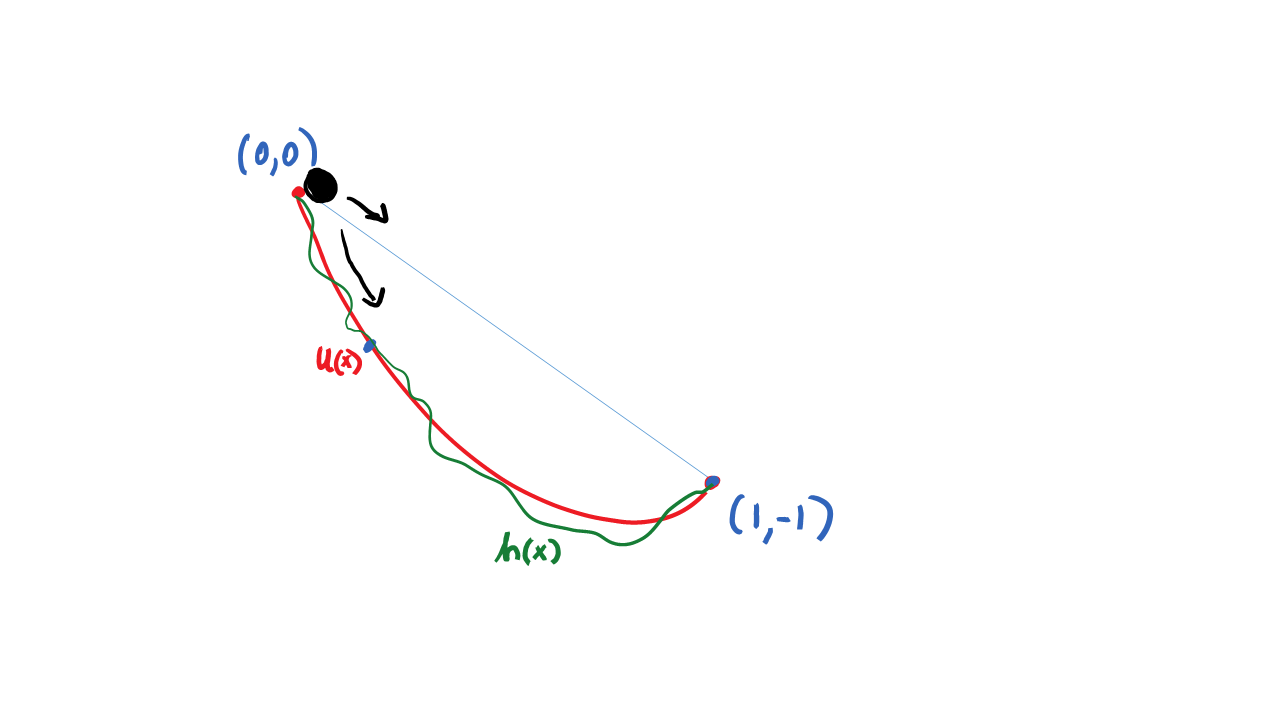
\includegraphics[width=4in]{fig3}\caption{The ``fastest'' curve\label{fig:rel-1}}
\end{figure}

\begin{proof}
Given a curve $u=u(x)$, the total travel time is
\[
T(u)=\int_{0}^{1}\frac{ds(x)}{v(x)}=\int_{0}^{1}\frac{\sqrt{1+(u'(x))^{2}}}{v(x)}dx
\]
where $ds$ is the arc length element and $v(x)$ is the velocity
at $x$. By conservation of energy, i.e., the gained kinetic energy
must equal the lost potential energy for every point along the curve,
we know that 
\[
\frac{1}{2}mv(x)^{2}=-mgu(x).
\]
Hence, we have $v(x)=\sqrt{-2gu(x)}$ and so 
\[
T(u)=\int_{0}^{1}\sqrt{\frac{1+(u'(x))^{2}}{-2gu(x)}}dx.
\]
Since $u$ is a \emph{shortest} curve, any local change in $u$ cannot
reduce the time, i.e., 
\[
DT(u)[h]=0
\]
for any change $h$ of the curve $u$. We next compute the directional
derivative of $T(u)$, i.e., $\frac{d}{dt}\vert_{t=0}T(u+th)$:
\begin{align*}
DT(u)[h] & =\int_{0}^{1}-\frac{1}{2}\frac{\sqrt{1+u'(x)^{2}}}{\sqrt{-2g}u(x)^{3/2}}\frac{d}{dt}u(x)dx+\int_{0}^{1}\frac{1}{2}\frac{2u'(x)}{\sqrt{-2gu(x)}\sqrt{1+u'(x)^{2}}}\frac{d}{dt}u'(x)dx.\\
 & =\int_{0}^{1}-\frac{1}{2}\frac{\sqrt{1+u'(x)^{2}}}{\sqrt{-2gu(x)}u(x)}h(x)dx+\int_{0}^{1}\frac{u'(x)h'(x)}{\sqrt{-2gu(x)}\sqrt{1+u'(x)^{2}}}dx.
\end{align*}
Note that the second term involves $h'(x)$. To change the term $h'(x)$
to $h(x)$, we use the integration by parts (with respect to $x$,
not $t$!):
\[
\int_{0}^{1}\frac{u'(x)h'(x)}{\sqrt{-2gu(x)}\sqrt{1+(u'(x))^{2}}}dx=\left[\frac{u'(x)h(x)}{\sqrt{-2gu(x)}\sqrt{1+(u'(x))^{2}}}\right]_{0}^{1}-\int_{0}^{1}\frac{d}{dx}\left(\frac{u'(x)}{\sqrt{-2gu(x)}\sqrt{1+(u'(x))^{2}}}\right)h(x)dx.
\]
Since the endpoints of the curve are fixed, we have $h(1)=h(0)=0$.
Hence, the first term on the right hand side is $0$. Continuing,
\begin{align*}
DT(u)[h]= & \int_{0}^{1}-\frac{1}{2}\frac{\sqrt{1+u'(x)^{2}}}{\sqrt{-2gu(x)}u(x)}h(x)dx-\int_{0}^{1}\frac{d}{dx}\left(\frac{u'(x)}{\sqrt{-2gu(x)}\sqrt{1+u'(x)^{2}}}\right)h(x)dx\\
= & \int_{0}^{1}-\frac{1}{2}\frac{\sqrt{1+(u'(x))^{2}}}{\sqrt{-2gu(x)}u(x)}h(x)dx-\int_{0}^{1}\frac{u''(x)}{\sqrt{-2gu(x)}\sqrt{1+u'(x)^{2}}}h(x)dx\\
 & +\int_{0}^{1}\frac{1}{2}\frac{u'(x)^{2}}{\sqrt{-2gu(x)}u(x)\sqrt{1+u'(x)^{2}}}h(x)dx\\
 & +\int_{0}^{1}\frac{u'(x)u'(x)u''(x)}{\sqrt{-2gu(x)}(1+u'(x){}^{2})^{3/2}}h(x)dx.
\end{align*}
Hence, we have $DT(u)[h]=\int_{0}^{1}a(x)h(x)dx$ where
\begin{align}
a(x)= & \frac{-1}{2}\frac{\sqrt{1+(u'(x))^{2}}}{\sqrt{-2gu(x)}u(x)}-\frac{u''(x)}{\sqrt{-2gu(x)}\sqrt{1+u'(x)^{2}}}+\frac{1}{2}\frac{u'(x)^{2}}{\sqrt{-2gu(x)}u(x)\sqrt{1+u'(x)^{2}}}\nonumber \\
 & +\frac{u'(x)u'(x)u''(x)}{\sqrt{-2gu(x)}(1+u'(x){}^{2})^{3/2}}.\label{brach_d}
\end{align}
Note that $a(x)$ is the gradient of $T$. Since $DT(u)[h]=0$ for
all $h(x)$, we have that $a(x)=0$ for all $x$. Multiplying both
sides of (\ref{brach_d}) by $2\sqrt{-2gu(x)}(1+(u'(x))^{2})^{3/2}u(x)$,
we have
\begin{align*}
0= & -(1+(u'(x))^{2})^{2}-2u(x)u''(x)(1+(u'(x))^{2})+u'(x)^{2}(1+(u'(x))^{2})+2u(x)u'(x)^{2}u''(x)\\
= & -1-u'(x)^{2}-2u(x)u''(x).
\end{align*}
\end{proof}

\subsection{Taking derivatives on both sides}

Suppose we have a function $f(x,y)$ and $g(x)$ such that $f(x,g(x))=0$.
The implicit function theorem shows that
\[
D_{x}f(x,g(x))+D_{y}f(x,g(x))Dg(x)=0
\]
where $D_{x}f$ is the Jacobian of $f$ with respect to $x$ variables
and $Dg(x)$ is the Jacobian of $g$. We note that the formula can
be obtained from taking derivative on both sides with respective to
$x$. Sometimes, taking derivatives on the both sides can greatly
simplify calculations. Here are some examples.
\begin{lem}
Consider $x_{t}=\argmin_{x\in\Rn}f_{t}(x)$ where $f_{t}$ are strictly
convex. Then, we have
\[
\frac{dx_{t}}{dt}=(\nabla^{2}f_{t}(x_{t}))^{-1}\nabla\frac{df_{t}}{dt}(x_{t}).
\]
\end{lem}

\begin{proof}
By the optimality condition, we have $\nabla f_{t}(x_{t})=0$. Taking
derivatives on both sides, we have
\[
\nabla^{2}f_{t}(x_{t})\frac{dx_{t}}{dt}+\nabla\frac{df_{t}}{dt}(x_{t})=0.
\]
Since $f_{t}$ are strictly convex, $\nabla^{2}f_{t}(x_{t})$ is positive
definite and is invertible. Hence, we have that the result.
\end{proof}
In section \ref{sec:IPM}, we used this to compute the derivative
of central path.

\subsection{Linearity of Expectation - the continuous version}

Often times one would like to compute the differential of a quantity
that is most appropriately expressed by an integral, and under mild
assumptions we can do so by simply swapping the integral and derivative,
i.e. for time differentiable and (Lebesgue) integrable $f(x,t)$ we
want to do
\[
\frac{d}{dt}\int_{\Omega}f(x,t)dx=\int_{\Omega}\frac{\partial}{\partial t}f(x,t)dx
\]
For example, we use this trick in deriving the Fokker-Planck equation
in gradient-based sampling. Fortunately, measure theory gives us the
dominated convergence theorem, a quick corollary of which tells us
we can perform the above trick as long as there exists integrable
$g:\Omega\rightarrow\R$ such that $\big|\frac{\partial}{\partial t}f(x,t)\big|\leq g(x)$
for all $x$. If we have $\Omega=\Rn$, then similar in nature to
integration by parts for divergence, the upper bound follows from
showing that the derivative of $f$ decays fast enough at infinity
(for absolutely continuous probability distributions with full support,
this is often the case).

\section{Solving optimization problems by hand}

In this section, we introduce the KKT condition and show how to use
it to solve optimization problem by hand.
\begin{thm}[Karush--Kuhn--Tucker theorem]
Consider the following optimization problem
\[
\min_{x\in\Omega}f(x)\text{ subject to }h_{i}(x)\leq0\text{ and }\ell_{j}(x)=0\text{ for all }i,j
\]
for some open set $\Omega$ and continuously differentiable functions
$f$, $h_{i}$ and $\ell_{j}$. If $x$ is a local minimum, $x$ satisfies
the KKT conditions:
\begin{itemize}
\item Stationary: $\nabla f(x)+\sum_{i}u_{i}\nabla h_{i}(x)+\sum_{j}v_{j}\nabla\ell_{j}(x)=0$
\item Complementary Slackness: $u_{i}h_{i}(x)=0$ for all $i$
\item Primal Feasibility: $h_{i}(x)\leq0$ and $\ell_{j}(x)=0$ for all
$i,j$
\item Dual Feasibility: $u_{i}\geq0$ for all $i$
\end{itemize}
We prove Holder's inequality as an example:
\end{thm}

\begin{fact}
For any vector $x,y\in\R^{n}$, we have $\|xy\|_{1}\leq\|x\|_{p}\|y\|_{q}$
for any $1\leq p\leq\infty$ and $1\leq q\leq\infty$ with $\frac{1}{p}+\frac{1}{q}=1$.
\end{fact}

\begin{proof}
By symmetries, it suffices to compute
\[
\max_{\|x\|_{p}\leq1}\sum_{i}x_{i}y_{i}
\]
for non-zero $y$. Now, we use the KKT theorem with $f(x)=-\sum_{i}x_{i}y_{i}$,
$h(x)=\|x\|_{p}-1$ and $\Omega=\R^{n}$. By the KKT conditions, for
any maximizer $x$, we have that
\begin{align*}
-\nabla f(x)+u\nabla h(x) & =0,\\
uh(x) & =0,\\
h(x)\leq0, & u\geq0.
\end{align*}
Note that $\nabla f(x)=y$ and $(\nabla h(x))_{i}=\frac{1}{p}\|x\|_{p}^{1-p}\cdot px_{i}^{p-1}=\|x\|_{p}^{1-p}\cdot x^{p-1}$.
From the stationary condition, we have
\[
y=u\|x\|_{p}^{1-p}\cdot x^{p-1}.
\]

To compute $u$, we note that $y$ is non-zero and hence $u\neq0$.
From the complementary slackness, we have $h(x)=0$ and hence $\|x\|_{p}=1$.
Therefore, we have
\[
y=u\cdot x^{p-1}.
\]
Hence, we have $1=\sum_{i}x_{i}^{p}=\sum_{i}(y_{i}/u)^{\frac{p}{p-1}}=\sum_{i}(y_{i}/u)^{q}$.
Hence, we have $u=\|y\|_{q}$ 

Now, we can compute $\sum_{i}x_{i}y_{i}$ as follows
\[
\sum_{i}x_{i}y_{i}=\sum_{i}(\frac{y_{i}}{u})^{\frac{1}{p-1}}y_{i}=\frac{1}{u^{1/(p-1)}}\sum_{i}y_{i}^{p/(p-1)}=\|y\|_{q}.
\]
\end{proof}

